\justifying

\section{Introduction}
Membrane technology has climbed to a paramount role in engineering applications such as water treatment,\cite{crittenden2012principles,baker2004overview}, gas separation,\cite{ismail2015membrane} energy storage,\cite{park2013renewable} and food packaging.\cite{figoli2010membranes} Recent works demonstrate that graphene could represent a valid alternative to traditional polymeric membranes\cite{li2013ultrathin,celebi2014ultimate} because of its mechanical strength,\cite{lee2008measurement} chemical stability,\cite{li2008processable} near frictionless water transport,\cite{konatham2013simulation,cohen2014water} and the potential to engineer well-defined surface pores and/or internal nanochannels.\cite{russo2012atom,goh2015all,yeh2015origin} However, a clear challenge is to understand how graphene nanoproperties affect the macroscopic performance of a device,\cite{chang2016guidelines} such as water filtration membranes.\\
With regard to nanoproperties, graphene-based membranes can be classified into two main groups: nanoporous graphene (NPG) and graphene oxide laminates (GOL).\cite{huang2015graphene} NPG is obtained by creating nanopores in a pristine graphene monolayer via ion bombardment and/or etching.\cite{o2014selective,o2015nanofiltration,cohen2016multilayer} GOL are synthesized by casting graphene oxide (GO) flakes on porous substrates. The flakes spontaneously arrange in an ordered fashion to form a laminate structure characterized by interconnected GO nanochannels.\cite{hung2014pressure}
The study of water transport in elemental carbon nanomaterials began in the mid-2000s, when fast (slip) water transport within nanometer-wide one-dimensional carbon nanotubes was reported.\cite{majumder2005nanoscale,joseph2008carbon} In 2012, the study of water transport in carbon materials expanded to two-dimensional (2D) carbon nano-architectures (such as NPG and subsequently GOL).\cite{boukhvalov2013origin,cohen2012water} GOL water transport has been modeled using molecular dynamics (MD), and results indicated a fast flow caused by the low wall friction of water within GO nanochannels or the presence of defects in the GO flakes.\cite{nair2012unimpeded,wei2014understanding} Experimental studies also observed GOL fast water transport,\cite{han2013ultrathin,Hu2013} although a clear consensus about the mechanism (low wall friction vs nanometer defects) has not yet been reached.\\
In this study, we provide insight into the influence of the properties of nanomaterials, \textit{e.g.}, GO surface chemistry, on the mechanism of water flow within GOL via a combination of
pressure-driven pure water permeability experiments and mesoscale lattice-Boltzmann (LB) fluid dynamics simulations. Ultrathin graphene oxide architectural laminates (GOAL, Fig.~\ref{Fig1_pap4}a) membranes were synthesized by vacuum filtration (VF) and then subsequently photoreduced by ultraviolet (UV) irradiation (in ambient or vacuum) or hydroiodic acid (HI) to finely tune nanomaterial chemistry (Fig.~\ref{Fig1_pap4}b). GO morphology was also controlled by varying the GO flake size via sonication prior to VF. The effect of GO surface chemistry and flake size on GOAL nanochannel architecture, e.g., interlayer spacing ($2h$) and tortuosity ($l$), was characterized by scanning electron microscopy (SEM), X-ray diffraction (XRD), and X-ray photoelectron spectroscopy (XPS). GOAL pure water permeability was determined in dead-end filtration mode, and mesoscale LB simulations were used to elucidate hydrodynamic phenomena.

\begin{figure}[t!]
  \centering
  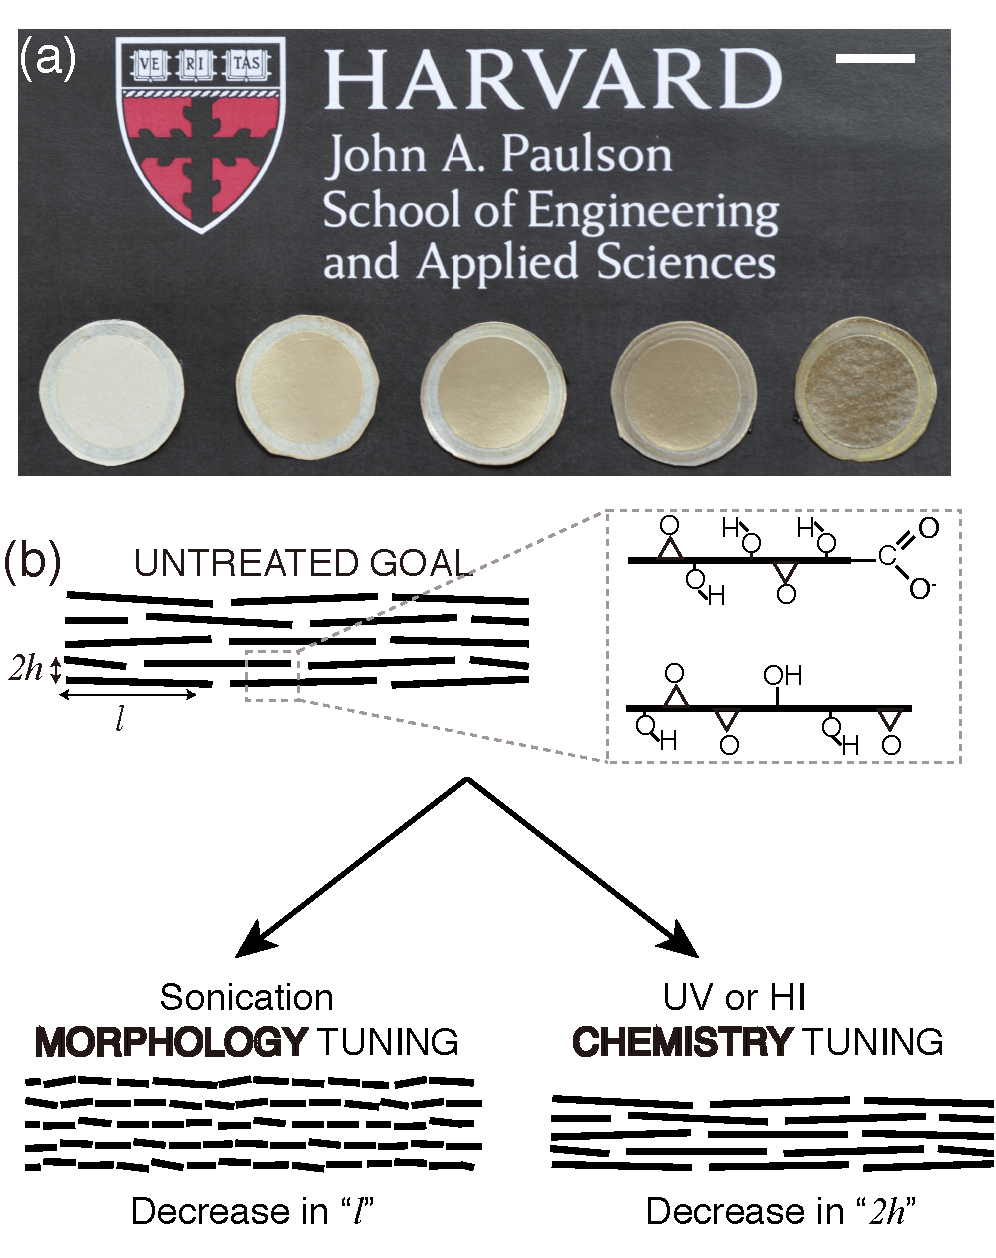
\includegraphics[width=4in]{paper4/Fig1.pdf}
  \caption{\textbf{GOAL membranes.} \textbf{(a)} Photographs of GOAL membranes obtained via chemical reduction increasing from left to right. The scale bar is 1 cm. \textbf{(b)} Two main dimensions ($2h$ and $l$) of the architecture of the nanochannels are independently modified with easy-to-implement techniques and are drawn to scale.}
  \label{Fig1_pap4}
\end{figure}

\section{Methods}

\subsection{Graphene Oxide Architectural Laminate Fabrication}
GO was synthesized by a modified Hummers method, and the detailed protocol can be found in our previous work.\cite{amadei2016fabrication} Postsynthesis, the GO solution was dispersed in ethanol at a concentration of 0.15 mg/mL. 1 mL of the GO solution was then dispersed in 20 mL of ethanol and vacuum-filtered onto a polyvinylidene difluoride (PVDF) membrane (\textit{Sterlitech}). In the case of sonicated GOAL (GOAL-son), prior to VF, the GO solution was bath sonicated for 23 min in a \textit{Branson} sonicator ($V=1.9$ L, maximal power $=80$ W, and $f=20$ kHz). UV-GOAL was obtained by exposing the VF membrane to UV light ($\lambda$=254 nm) in ambient air. Vacuum UV treatment was performed in a \textit{TTP4-1.5K} Probe Station (\textit{LakeShore}) at 10\textsuperscript{-7} Torr. HI treatment was performed by immersing the GOAL for 1 min in an aqueous concentrated HI solution (55\%) at 50 \textdegree C. The membrane was then washed with 50 mL of deionized water.

\subsection{Graphene Oxide Architectural Laminate Characterization}
\textbf{Scanning electron microscopy (SEM):} The morphology of the bare PVDF, GO flakes, and GOAL was characterized using a \textit{Zeiss ULTRA} Field Emission Scanning Electron Microscope with an In-lens secondary electron detector. The working distance was $4-5$ mm, and the acceleration voltage was 4 kV. The GO flake area was determined using \textit{ImageJ} SEM analysis. In (Fig.~\ref{Fig2_pap4}), the \textit{Adobe Photoshop} blend option was used at the border between bare PVDF and GOAL.\\
\textbf{X-Ray photoelectron spectroscopy (XPS):} GOAL chemistry was analyzed by a \textit{Thermo Scientific K-Alpha} XPS instrument (ESCA) with X-rays generated by a 12 kV electron beam with a spot size of 400 $\mu$m. The O/C ratio and peak deconvolution were quantified by \textit{Thermo Scientific Avantage} software, and then convert to mass ratio by using C and O molecular weights. The XPS instrumental error for atomic composition is $\pm$1\%, and the accuracy of the C1s peak fitting is $\pm$2\%.\\
\textbf{Atomic force microscopy (AFM):} GOAL and bare PVDF morphology was characterized with an \textit{Asylum Cypher} atomic force microscope using an \textit{Olympus 200TS} cantilever (resonant frequency of $\approx150$ kHz). The images were acquired in amplitude modulation mode,\cite{Paulo2002} and the tip size was constantly monitored.\cite{santos2012method}\\
\textbf{X-ray diffraction (XRD):} The GOAL crystallographic structure was analyzed with a \textit{Bruker D8} instrument equipped with a 2D \textit{VANTEC-500} detector. The spectra were recorded by the integration of the 2D images via EVA software. Depending on the sample, the integration time was between 600 and 1200 s. Note that the bare PVDF XRD spectrum is characterized by peaks that could overlap with that of GO. Thus, to increase the signal-to-noise ratio, the GOAL was cast and reduced on a porous alumina oxide ($d\textsubscript{pore}=200$ nm) from \textit{Whatman}.\\
\textbf{Static contact angle (SCA):} The SCA measurements were completed with a \textit{Rame-Hart 190} contact angle goniometer under ambient conditions. SCA were measured using 5 $\mu$L droplets and the data refer to the average of 5 measurements obtained with the \textit{Drop AnalysiseDroSnake} plugin in \textit{ImageJ}.\\
\textbf{Raman spectroscopy:} Raman spectra were acquired using a \textit{WITec} Confocal Raman Microscope. The laser wavelength was 532 nm and the signal was acquired using a 0.3 s integration time of at least 10 spectra.
\subsection{Lattice-Boltzmann Simulations}
The numerical simulations are based on the LB method adapted using a novel Langevin-like frictional force to account for the GO-water H-bonding interactions. Because the LB method has largely been documented in the literature,\cite{aidun2010lattice,succi2001lattice} in the following we briefly introduce the LB model and the heterogeneous Langevin frictions term to account for the frictional interaction of oxy-functional groups on water molecule transport as described in eqn~(\ref{eqn1_pap4}): 
\begin{equation}
f_i(x+c_i\Delta t,t+\Delta t) = f_i(x,t)+\dfrac{1}{\tau}[(f_i^{eq}(\rho, \rho u)-f_i(x,t)] + \Delta f 
 \label{eqn1_pap4}
\end{equation}
where $f_i$ is the probability distribution function at position $x$ and time $t$ with a lattice-constrained velocity $c_i$, where index i runs over the nine directions of the lattice, $f_i^{eq}$ is a proper expansion of the Maxwell-Boltzmann distribution that can be expressed as a function of density $\rho$ and linear momentum $\rho u$, and the frictional force, $\Delta f$, is described in eqn~(\ref{eqn2_pap4}.
\begin{equation}
\Delta f \sim -\rho \gamma (y)u 
 \label{eqn2_pap4}
\end{equation}
where the function $\gamma$ is described in eqn~(\ref{eqn3_pap4}:
\begin{equation}
\gamma (y) \sim \gamma_0 [exp(-\dfrac{y}{w})]
 \label{eqn3_pap4}
\end{equation}
where $w=0.2$ is the representative size of the protruding oxy-functional groups and $\gamma_0$ is a characteristic water-hydroxyl collision frequency taken to be equal to 70 ps\textsuperscript{-1}.\cite{pastor1988analysis} This comes from the conversion between LB and physical units, namely, $\gamma_{phys}=\gamma_{LB}/dt$, where $dt=3\times10^{-15}$ s. Thus, the value of $\gamma_0$ has been chosen to match the characteristic water-water collision frequency value, which can be determined via MD simulations by monitoring the velocity autocorrelation function.\cite{pastor1988analysis} Wall function $H_L(y)$ takes a value of 1 when $0<y<\delta$ and 0 elsewhere. Likewise, $H_R(y)=1$ for $2h−δ<y<2h$ and 0 elsewhere.\\
Assuming the GOL structure to be symmetric and periodic,\cite{han2013ultrathin} we consider only two nanochannels out of the full device, characterized by a width equal to the spacing of GO ($2h$) and a length equal to l. A similar geometry has been recently employed to investigate the permeation of water through graphene-based membranes by means of MD simulations.\cite{muscatello2016optimizing} These two channels are connected via two openings of half the width of the inlet/outlet pores (Fig.~\ref{figS1_AppC} in the Appendix C). The boundary conditions at the left-right and top-bottom surfaces are periodic, to simulate the proximity of two adjacent GO layers. If applied, at solid walls, the molecules experience the Langevin frictional force previously described. The grid resolution is 10000 x 20, corresponding to a flake length of $10^{-6}$m.\\
The physical idea behind the Langevin frictional force is to account for the complex water-GO surface molecular interactions at a coarse-grain level, whereby all atomistic details are channeled into parameters  $\gamma_0$ and $w$. Note that the frictional force is considered to be uniform along the nanochannels. However, further studies could investigate the influence of heterogeneous frictional force characterized by regions with lower and/or higher friction, which would represent heterogeneity in the distribution of the oxy-functionalities. Refer to ref.\cite{montessori2017extended} for more details.
\subsection{Permeability Measurements}
The permeability tests were performed in a custom-made dead-end filtration system (Fig.~\ref{figS2_AppC} in the Appendix C). The filtration system includes a 3.1 L reservoir (\textit{e.g.}, pressure pot from \textit{Alloy Product Corp.}) allowing large-volume experiments to be performed. The pressure was regulated with a pressure gauge (\textit{Ingersoll}). The pure water permeability was evaluated by monitoring the permeate volume with a \textit{Sartorious} laboratory balance every 30 min. The pure water permeability was then obtained by dividing the flow rate by the applied pressure and membrane area.
\section{Results and Discussion}
\subsection{Tuning of Graphene Oxide Dimensions}
GOAL were cast on a PVDF microfiltration membrane via VF, and their morphology was determined by SEM (Fig.~\ref{Fig2_pap4}). In the right portion of Fig.~\ref{Fig2_pap4}a, the bare PVDF membrane is characterized by a flowerlike structure with a pore size of $310\pm126$ nm. After VF, the GOAL homogeneously coats the PVDF (Fig.~\ref{Fig2_pap4}a, left), but the flowerlike structure of the PVDF is still observed (inset in Fig.~\ref{Fig2_pap4}a), because of the ultrathin ($47\pm6$ nm) GOAL (mass and SEM analysis), which is highlighted by a cross-sectional image (Fig.~\ref{Fig2_pap4}b). Morphology conservation is important for membranes because specific nano- and micro-morphology affects fouling.\cite{hu2016organic} GOAL morphology and thickness are also corroborated by AFM images (Fig.~\ref{Fig2_pap4}c-d and (Fig.~\ref{figS3_AppC} in the Appendix C). In particular, the images are taken at the boundary (highlighted with a black line) between the GO and the bare PVDF. From the topography image (Fig.~\ref{Fig2_pap4}c), again it is possible to notice that the thin GO layer preserves the flowerlike structure of the PVDF membrane. Important information can also be derived from the AFM phase image (Fig.~\ref{Fig2_pap4}d), which is affected by the chemistry of the sample.\cite{Paulo2002} Thus, heterogeneity between GOAL and PVDF chemistry can be easily recognized.\\
\begin{figure}[t!]
  \centering
  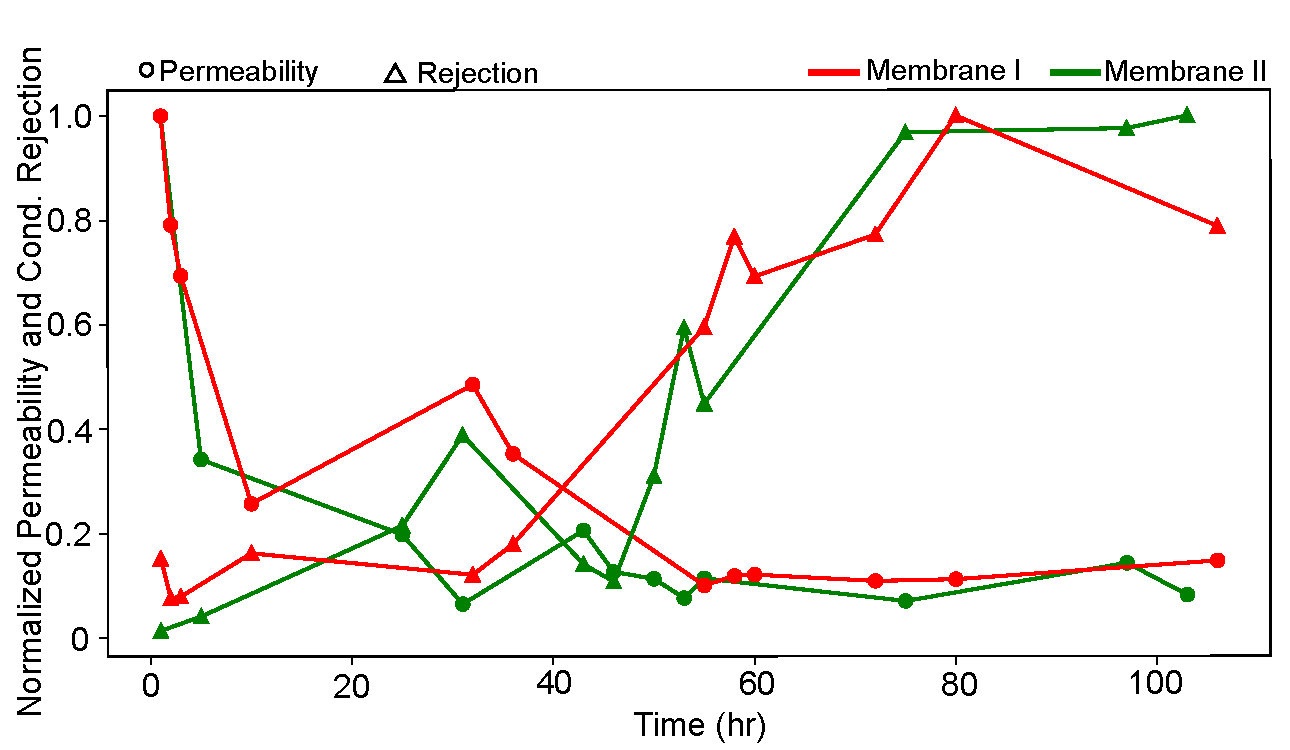
\includegraphics[width=5in]{paper4/Fig2.pdf}
  \caption{\textbf{GOAL morphology via SEM and AFM.} \textbf{(a)} Areal top-down and \textbf{(b)} cross-sectional images of GOAL membranes obtained via SEM. \textbf{(c)} Topography and \textbf{(d)} phase image acquired at the boundary between the GOAL and the bare PVDF via AFM. The boundary between the two regions is highlighted with a solid black line.}
  \label{Fig2_pap4}
\end{figure}
The GOAL and PVDF are then subjected to reductive treatment, such as UV irradiation ($15-1440$ min). Previous reports indicate that the effects of UV irradiation\cite{gengler2013revealing,xing2014uv,guo2009green} on GO will depend on the environment (\textit{e.g.}, water or air) and can dictate whether GO reduction occurs.\cite{li2014tuning} In this work, we for the first time explore the UV reduction of GO in vacuum, which may reduce the extent of photochemical degradation and increase conductivity.\cite{hou2015photochemical} The evolution of the GOAL XPS C1s spectrum with UV irradiation time is shown in Fig.~\ref{Fig3_pap4}a. After 1440 min, GOAL graphitization is indicated by an increase in the carbon−carbon (C-C and C=C, binding energy of 285 eV) bond peak percentage of total C bonds from $28\pm2$ to $71\pm2$\%. Correspondingly, the relative carbon-oxygen single-bond peak intensity, such as hydroxide (C-OH, 287 eV), decreases from $69\pm1$ to $14\pm1$\%, and the carbon-oxygen double-bond peak intensity (C=O, 289 eV) increases by 5\%. The oxygen/carbon mass (\textit{i.e.}, O/C) ratio decreases from $72\pm2$ to $35\pm2$\% from the untreated GOAL to the 1440 min UV-irradiated GOAL, respectively. The XPS characterization data are summarized in Table~\ref{tblS1_AppC}, and eqn~(\ref{eqn4_pap4} represents a possible chemical reaction during UV irradiation in which an epoxide is photolyzed to a C=C bond:
\begin{equation}
\schemestart
  {\ce{C-O-C} + \ce{hv} \arrow{->}\ce{-C=C-} + \ce{O2_{(g)}}} 
\schemestop
 \label{eqn4_pap4}
\end{equation}
The GOAL XRD spectrum as a function of UV irradiation time is shown in Fig.~\ref{Fig3_pap4}b All spectra display a peak corresponding to the GOAL interlayer spacing ($2h$) (Fig.~\ref{Fig1_pap4}b). The interlayer spacing is quantitatively correlated to the GOAL oxygen content indicating basal plane oxy-groups mediate GOAL interlayer spacing at the angstrom level. Specifically, UV reduction of oxy-functional groups results in an XRD peak shift of 2.7 {\AA} or an 25\% decrease in $2h$, 7.9 {\AA} for untreated GOAL to 6.2 {\AA} for GOAL after UV treatment for 1440 min. Elemental carbon reduction has been observed to be dependent on the environment;\cite{Pei2012} thus, we compared the reduction via UV irradiation in vacuum versus ambient air. The GOAL O/C mass ratio after UV irradiation for 60 min in vacuum is similar to that after 360 min in air, indicating significantly faster reduction kinetics, and the final O/C mass ratio after 1440 min is $35\pm2$\% and $46\pm2$\% for UV in vacuo and air, respectively (see Table~\ref{tblS1_AppC} in the Appendix C). GOAL UV irradiation in air results in slower reduction likely because of ambient O\textsubscript{2} propagating reactions with GO surface radicals and slower removal of UV-produced gaseous radicals (eqn~(\ref{eqn4_pap4}), which is similar to phenomena during thermal reduction of GO.\cite{bagri2010structural,mattevi2009evolution} Correspondingly, UV GOAL treatment in air results in broader XRD peaks indicating a more disordered structure than that after UV treatment in vacuum. For example, the full widths at half-maximum after UV treatment for 60 min are $\approx1.2$\textdegree \ and  $\approx1.8$\textdegree \ for vacuum and ambient air, respectively (Fig.~\ref{figS4_AppC}b in the appendix C). Alternatively, the GOAL were also reduced by concentrated HI at 50 \textdegree C for 1 min. HI reduces the GOAL to a greater extent than UV, in accordance with previous reports,\cite{su2014impermeable,pei2010direct} resulting in an O/C mass ratio of $20 \pm 2$\% and an interlayer spacing of 5.5 {\AA} (Fig.~\ref{figS5_AppC} in the Appendix C). Again, HI reduction of GOAL oxy-functional groups led to a decrease in interlayer spacing and indicated a possible relationship between the two variables. Although other studies investigated the effect of GO reduction on oxygen content and spacing,\cite{andrikopoulos2014effect,alhadhrami2016thermal} a quantitative relationship between these parameters has not been previously reported. GOAL interlayer spacing ($2h$) as a function of oxygen content (O) is displayed in Fig.~\ref{Fig3_pap4}c  and well fit ($\mathbb{R}^{2}> 0.99$) by an exponential rise to a maximal GO interlayer spacing:
\begin{equation}
2h = a-b(e^{(-cO)})
 \label{eqn5_pap4}
\end{equation}
\begin{figure}[t!]
  \centering
  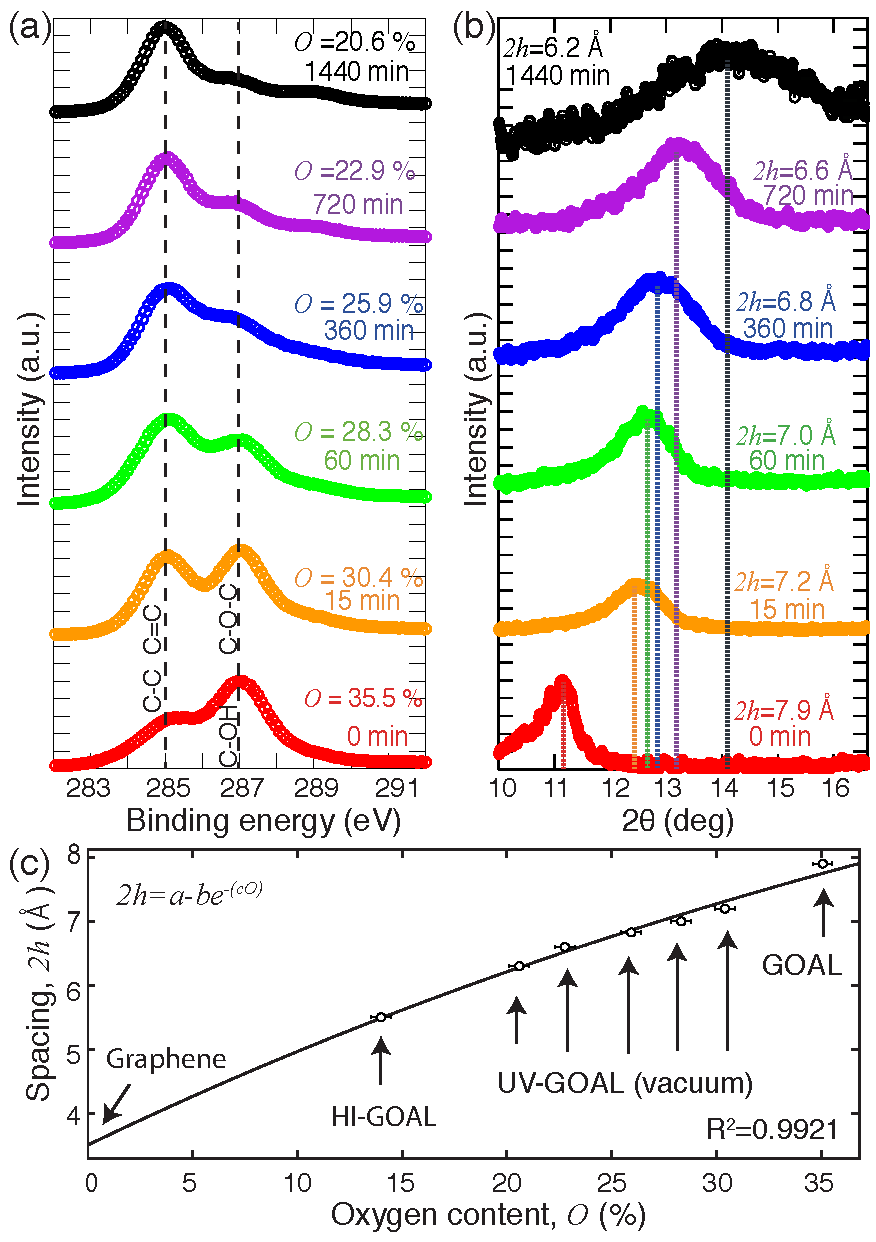
\includegraphics[width=5in]{paper4/Fig3.pdf}
  \caption{\textbf{GOAL interlayer spacing as a function of oxygen content.} \textbf{(a)} XPS and \textbf{(b)} XRD time-dependent spectra for UV-irradiated GOAL membranes in vacuum. The XRD full width at half-maximum peak is equal to 0.7\textdegree, 1\textdegree, 1.2\textdegree, 1.3\textdegree, 2\textdegree, and 3.5\textdegree \  for irradiation times of 0, 15, 60, 360, 720, and 1440 min, respectively. \textbf{(c)} The GOAL interlayer spacing as a function of GO oxygen content can be fitted with an exponential rise to maximal GO interlayer spacing. In the equation, a-c are empirical coefficients with values of 29.6, 26, and 0.004, respectively.}
  \label{Fig3_pap4}
\end{figure}
where $a$, $b$, and $c$ are empirical coefficients with values of 29.6, 26, and 0.004, respectively. The difference in coefficients a and b that defines the spacing for pristine graphene (\textit{i.e.}, $O = 0$) yields $2h = 3.63 $ {\AA}, which is similar to the theoretical spacing (3.4 {\AA}) supporting the theoretical reliability of the trend in Fig.~\ref{Fig3_pap4}c. In the case of completely oxidized GO ($O = 100$; one $O$ atom for one C atom), eqn~(\ref{eqn5_pap4} yields $2h = 12.2$ {\AA}, the upper limit for GO spacing. Note that a GO with an O/C mass ratio of $\geq1$ has never been obtained to the best of our knowledge, and experiments that aimed to investigate the oxidation of GO achieved a maximum of $\approx60$\% carbon bonds oxidized.\cite{ying2014plane} The small $c$ value indicates that large changes in O will result in subangstrom variation in GOAL interlayer spacing. The relation in eqn~(\ref{eqn5_pap4}  has potential to significantly decrease GOL characterization time by performing a single characterization (\textit{e.g.}, XPS or XRD) to determine both oxygen content and interlayer spacing. Note that eqn~(\ref{eqn5_pap4} currently applies to our synthesized GOAL, but deviations from this may be expected due to alternative casting techniques and/or varying GO properties (\textit{e.g.}, flake size and/or oxy-functional group content and/or distribution).
GOAL reduction results in a corresponding reduction of GO nanochannel spacing. However, it is also possible to rationally modify the length ($l$) of the nanochannels (Fig.~\ref{Fig1_pap4}, right) by ultrasonic irradiation of the GO solution before VF casting.\cite{amadei2016fabrication} For example, the GO flake area decreased by more than 1 order of magnitude, from $52.2\pm18.9$ to $1.3\pm0.4$ $\mu$m\textsuperscript{2} (Fig.~\ref{figS6_AppC} in the Appendix C), after bath sonication for 23 min corresponding to a decrease in $l$ by a factor of $\approx7$, assuming a square flake. Note that the modifications of $2h$ and $l$ are not interdependent as it is possible to modify one dimension without affecting the other (Fig.~\ref{figS7_AppC}). In other words, sonication does not affect the spacing ($2h$) and chemical modification does not affect the morphology of the flakes ($l$).\\
\subsection{Graphene Oxide Architectural Laminate Permeability}
Once we had demonstrated the ability to tune primary GOAL dimensions ($2h$ and $l$) by exploiting GO metastability, the GOAL water permeability as a function of GO nanoscopic properties was investigated. Attention was focused on eight GOAL: (i and ii) untreated GOAL (0-GOAL and 0-GOAL-son), (iii and iv) 15 min UV-irradiated GOAL in vacuum (15-GOAL and 15-GOAL-son), (v and vi) 360 min UV-irradiated GOAL in vacuum (360-GOAL and 360-GOAL-son), and (vii and viii) HI-treated GOAL (HI-GOAL and HI-GOAL-son). Note that -son refers to membranes obtained by casting a GO solution that was sonicated and, thus, characterized by a smaller GO flake size. Sonication does not introduce significant changes into the defect density as corroborated by Raman image analysis (see Appendix C). The pure water permeabilities were obtained via dead-end filtration (Fig.~\ref{figS2_AppC} in the Appendix C) and are summarized in Fig.~\ref{Fig4_pap4}.

\begin{figure}[h!]
  \centering
  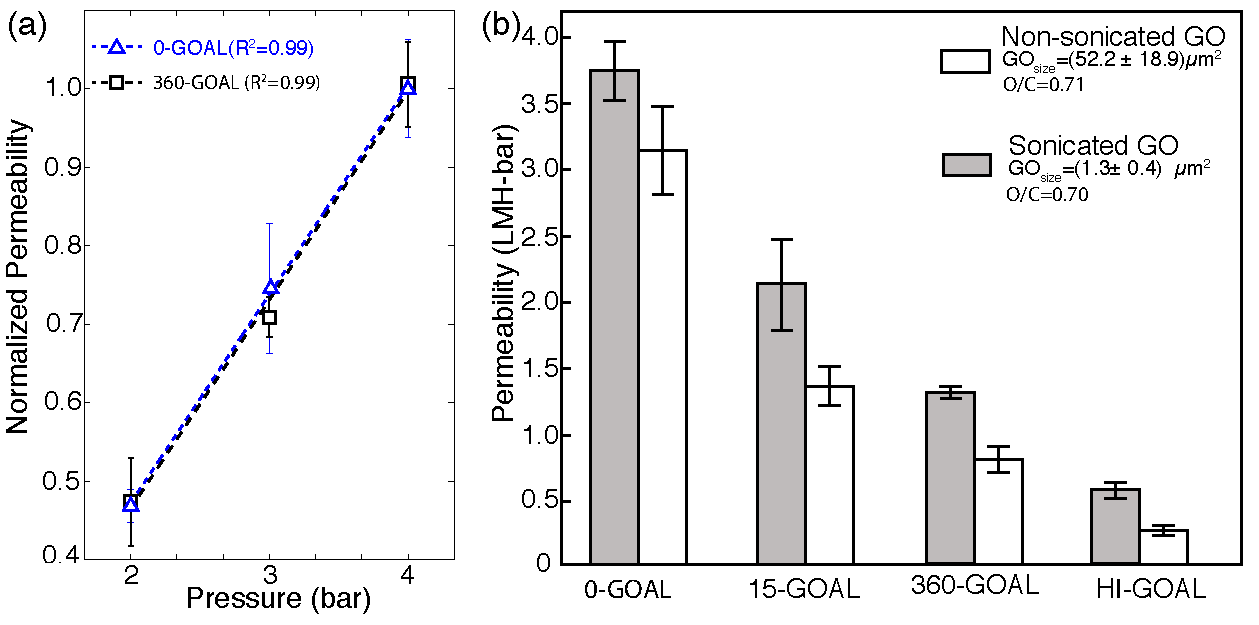
\includegraphics[width=6in]{paper4/Fig4.pdf}
  \caption{\textbf{GOAL pure water permeability.} \textbf{(a)} Darcy behavior of the UV-treated GOAL membranes in vacuum. \textbf{(b)} Permeability of eight GOAL membranes. Each permeability was evaluated in at least duplicate.}
  \label{Fig4_pap4}
\end{figure}
The normalized flux for two membranes [0-GOAL (blue) and 360-GOAL (black)] at three pressures (2, 3, and 4 bar) is presented in Fig.~\ref{Fig1_pap4}a. The water flux is linearly dependent on the applied pressure indicating Darcy behavior. These data are also supported by the decrease in permeability with an increase in GOAL thickness (Table~\ref{tblS2_AppC}). In the Darcy hydrodynamic regime, water transport follows the no-slip condition.\cite{thomas2009water,suk2010water} The permeability in LMH-bar (i.e., liters per square meter per hour per bar) for the eight GOAL membranes is displayed in Fig.~\ref{Fig4_pap4}b. In terms of absolute values, the permeability varies from $3-4$ to $0.25-0.75$ LMH-bar, in accordance with values reported for reduced ultrathin GO membranes on polymer substrates.\cite{han2013ultrathin,Hu2013,hu2016organic,hu2014layer} Although higher values (tens of LMH-bar) of permeability have been reported for GO membranes, these values may be related to the presence of defects or GO nanochannels larger than those observed here because of the reduction of the GO membranes in air.\cite{xia2015ultrathin,qiu2011controllable} Increased permeability ($>100$ LMH-bar) can also be achieved by intercalating GO with high-aspect ratio nanostructures such as rods.\cite{goh2015all,huang2013ultrafast} Discrepancies between permeability values reported in Fig.~\ref{Fig1_pap4}b and previous literature values could also emerge from the fact that previous studies did not evaluate the membrane performance under steady-state conditions (always lower than the initial permeability).\cite{amadei2016increase} For example, the time-dependent permeate volume (Fig.~\ref{figS8_AppC}) shows that the GOAL flow rate decreases with time until reaching steady-state conditions at $\approx700$ min, similar to the case for polymer membranes, and the GOAL initially compresses after pressure is applied likely because of GO flake rearrangement.\cite{huang2013ultrafast,huang2013salt} For example, 0-GOAL have an initial permeability $3-4$-fold greater than the steady-state permeability.\\
A clear decrease in GOAL permeability is also observed upon GO chemical reduction (Fig.~\ref{Fig1_pap4}b). For example, a $6-7$-fold reduction in permeability is observed for HI-GOAL (0.54 LMH-bar) compared to 0-GOAL (3.77 LMH-bar) even though there is only a 50\% reduction in $2h$. Increasing the UV irradiation time also leads to a decrease in GOAL permeability [2.11 and 1.29 LMH-bar for 15-GOAL ($2h = 7.2$ {\AA}) and 360-GOAL ($2h = 6.8${\AA}), respectively]. In summary, permeability is predominantly related to a decrease in GO interlayer nanochannel spacing ($2h$), which in turn is related to the extent of GO chemical reduction, and there is little effect from reducing GO length ($l$) by sonication.\\
The permeability decrease with reduction indicates that the process does not create macroscopic defects (i.e., holes) in the GOAL structure, which would result in an increased permeability,\cite{qiu2011controllable} and instead favors an increase in the extent of interlayer $\pi-\pi$ GO interactions and a reduction in nanochannel spacing ($2h$).\cite{yang2009chemical} Enhanced $\pi-\pi$ interaction is confirmed by Raman spectroscopy as the D/G peak intensity ratio (I\textsubscript{D}/I\textsubscript{G}) decreases with an increase in UV irradiation time, confirming the restoration of the graphitic domains via GOAL reduction (Fig.~\ref{figS9_AppC)}). I\textsubscript{D}/I\textsubscript{G} is 1.1 for untreated GO and decreases to 0.95 and 0.90 for GO UV after irradiation in vacuum for 15 and 720 min, respectively. GOAL reduction also increases hydrophobicity, with the static contact angle (SCA) increasing from $55.6\pm1.2$\textdegree\ (0-GOAL) to $77.2\pm2.1$\textdegree\ (HI-GOAL).\cite{moon2010reduced,lee2013route} In particular, the increase in hydrophobicity is exponentially dependent on the extent of GO reduction ( Fig.~\ref{Fig5_pap4}) according to eqn~(\ref{eqn6_pap4}:
\begin{equation}
2h = g-d(e^{(-fO)})
 \label{eqn6_pap4}
\end{equation}
A theoretical basis of this trend is confirmed by the fact that eqn~(\ref{eqn6_pap4} yields a SCA of 82.1\textdegree\ for pristine graphene/graphite ($O = 0$\%), which is corroborated by several experimental and simulation reports.\cite{amadei2014time,kozbial2014understanding,li2013effect} The increase in hydrophobicity may also affect the water transport and thus GOAL permeability.
\begin{figure}[h!]
  \centering
  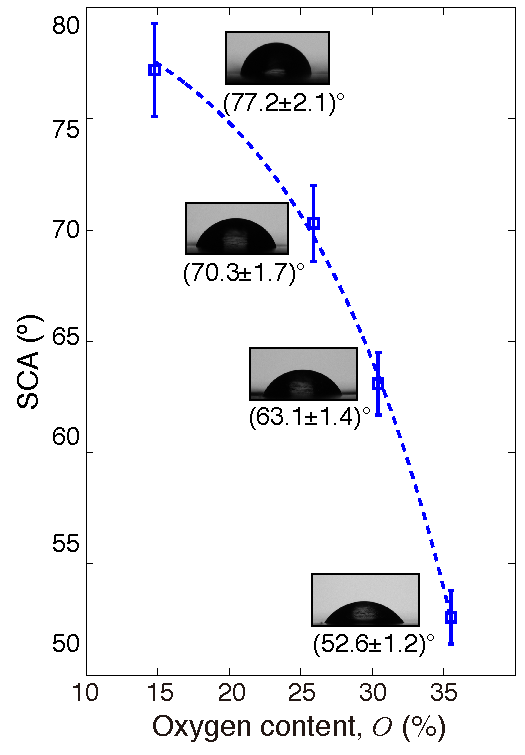
\includegraphics[width=3in]{paper4/Fig5.pdf}
  \caption{\textbf{GOAL SCA vs oxygen content.}}
  \label{Fig5_pap4}
\end{figure}
For comparison, sonication increased GOAL permeability by only $0.6\pm0.3$-fold (gray bars,Fig.~\ref{Fig4_pap4}b), even though $l$ decreased by $\approx7$-fold. The permeability increase is related to the decrease in membrane tortuosity caused by a decrease in the length ($l$) of the GO. Considering HI-GOAL, it is of note that a $2h$ decrease of 30\% (from 7.9 to 5.5 {\AA}) results in an $\approx90$\% decrease in water permeability; in contrast, a decrease of $\approx700$\% in $l$ ($\approx7$ to $\approx1$ $\mu$m) resulted in an increase of only $\approx100$\% in the water permeability, suggesting a 2D transport regime that does not follow Hagen-Poiseuille flow.\\
The change in permeability ($\Delta k$) was divided by the respective change in the dimension for the two scenarios ($\Delta2h$ and $\Delta l$) to produce $\Delta k_l$ and $\Delta k_{2h}$ normalized to the unmodified GOAL, where subscripts indicate the dimension in question. Note that the $\Delta2h$  values refer to a dry state whereas the $\Delta k$ values refer to a hydrated state. It is known that upon immersion in water the GO spacing can increase $20-25$\%.\cite{talyzin2014structure} However, the GO spacing decreases after the pressure is applied (decrease in permeability in Fig.~\ref{figS7_AppC}; thus, monitoring of $2h$ when the membrane is in operation is challenging. In our recent perspective, we discuss the need of a characterization tool, which can measure the spacing of the GO membrane when in operation.\cite{amadei2016increase} To overcome this challenge, normalized coefficients (\textit{i.e.}, $\Delta k_{2h}$) based on relative and not absolute values, were used. This choice is also supported by the fact that both the reduced and non-reduced GOAL swelled to a similar magnitude ($20-25$\% increase) upon being hydrated (Fig.~\ref{figS10_AppC}. The $\Delta k_{2h}$ values range from 2.80 to 6.35, whereas $\Delta k_{l}$ values range from 0.02 to 0.1 (Table~\ref{tblS3_AppC} and Table~\ref{tblS4_AppC}). The order of magnitude difference between the two ranges highlights that the characteristic dimension dominating permeability is $2h$, which is controlled by the GO chemistry, whereas in comparison, $l$ has a limited effect on permeability.\\
To gain a deeper understanding of the GOAL water transport mechanism, an LB approach augmented with a novel Langevin-like frictional forcing term between water molecules and the GO nanochannel basal plane oxy-functional groups via H-bonding was employed (Fig.~\ref{Fig6_pap4}). The model geometry and the characteristic water flow path within the GO nanochannel are displayed in Fig.~\ref{Fig6_pap4}a. Of note is the large simulation domain (thousands of square nanometers), which would be computationally costly for simulation tools currently used to evaluate water transport within GO nanochannels (\textit{e.g.}, MD or first-principle calculations).\cite{boukhvalov2013origin,wei2014understanding,wei2014breakdown} The $\Delta k_{2h}$ versus GO nanochannel height variation ($\Delta2h$) is plotted in Fig.~\ref{Fig6_pap4}b. Simulations were performed for four different interlayer spacings of 7.2, 6.7, 6.3, and 6.1 {\AA} and for a flake size equal to the size of the sonicated flake ($\approx1$ $\mu$m). From the simulation, $\Delta k_{2h}$ decreases with a decrease in GO interlayer spacing from 5 ($2h = 7.2$ {\AA}) to 3 $(2h = 6.$1 {\AA}), in agreement with experimental range ($2.80 < \Delta k_{2h} < 6.35$). The simulations support the trend of a decreasing permeability with a decrease in GOAL interlayer spacing. Of note for both experimental and simulation outputs, the smallest variations in the spacing ($<10$\%) lead to the largest normalized variations in permeability ($>5$). This spacing variation could also be achieved by unintentional reduction of the GOAL (\textit{i.e.}, prolonged exposure to sunlight) and highlights how GO metastability\cite{yeh2015origin,kim2012room}may affect the macroscopic performance of GO-based applications.
\begin{figure}[h]
  \centering
  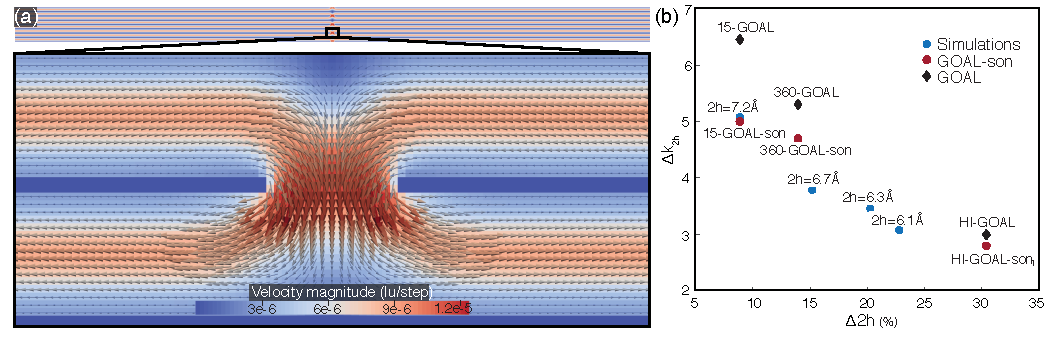
\includegraphics[width=6in]{paper4/Fig6.pdf}
  \caption{\textbf{LB simulations.} \textbf{(a)} GOAL geometry setup employed in the simulations and a magnification of the velocity field inside. \textbf{(b)} Normalized permeability vs interlayer spacing change for experimental and simulation outputs. The interlayer spacing change is normalized to the largest spacing value (7.9 {\AA}).}
  \label{Fig6_pap4}
\end{figure}
In summary, we report on methods for independent fine control of GOAL nanodimensions (length and height of the GOAL nanochannels) and surface chemistry via easy-to- implement techniques such as photoreduction and bath sonication. In particular, the permeability tests highlight that GO interlayer spacing is the predominant dimension dictating GOAL water transport, although hydrophobicity effects may also need to be taken into account. 

\section{Conclusions}
The environmental implications of this study center on GO metastability and are two-fold. First, the GO photochemical oxidation state is highly dependent on the surrounding medium and on the time of exposure. For the performance of GOAL in environmental applications to be consistent with time, it is paramount to use a stable GO material with limited redox activity. In other words, the GO should be reduced in a controlled manner before being implemented and utilized in a controlled environment. Second, GO metastability may be exploited to tailor the specific nanoproperties, which will affect the macroscopic GOAL properties. Thus, tuning of GO chemistry and morphology will allow GOAL to be a versatile material utilized for a range of environmental applications.\\
The results presented here offer fundamental knowledge about simple methods for controlling GO properties and thus the ability to rationally design and construct GOAL membranes. This deep understanding of the effect of GO nanoproperties on membrane performance represents a major challenge for the widespread use of GO in separation processes.

